% Options for packages loaded elsewhere
\PassOptionsToPackage{unicode}{hyperref}
\PassOptionsToPackage{hyphens}{url}
\PassOptionsToPackage{dvipsnames,svgnames,x11names}{xcolor}
%
\documentclass[
  letterpaper,
  DIV=11,
  numbers=noendperiod]{scrartcl}

\usepackage{amsmath,amssymb}
\usepackage{lmodern}
\usepackage{iftex}
\ifPDFTeX
  \usepackage[T1]{fontenc}
  \usepackage[utf8]{inputenc}
  \usepackage{textcomp} % provide euro and other symbols
\else % if luatex or xetex
  \usepackage{unicode-math}
  \defaultfontfeatures{Scale=MatchLowercase}
  \defaultfontfeatures[\rmfamily]{Ligatures=TeX,Scale=1}
\fi
% Use upquote if available, for straight quotes in verbatim environments
\IfFileExists{upquote.sty}{\usepackage{upquote}}{}
\IfFileExists{microtype.sty}{% use microtype if available
  \usepackage[]{microtype}
  \UseMicrotypeSet[protrusion]{basicmath} % disable protrusion for tt fonts
}{}
\makeatletter
\@ifundefined{KOMAClassName}{% if non-KOMA class
  \IfFileExists{parskip.sty}{%
    \usepackage{parskip}
  }{% else
    \setlength{\parindent}{0pt}
    \setlength{\parskip}{6pt plus 2pt minus 1pt}}
}{% if KOMA class
  \KOMAoptions{parskip=half}}
\makeatother
\usepackage{xcolor}
\setlength{\emergencystretch}{3em} % prevent overfull lines
\setcounter{secnumdepth}{-\maxdimen} % remove section numbering
% Make \paragraph and \subparagraph free-standing
\ifx\paragraph\undefined\else
  \let\oldparagraph\paragraph
  \renewcommand{\paragraph}[1]{\oldparagraph{#1}\mbox{}}
\fi
\ifx\subparagraph\undefined\else
  \let\oldsubparagraph\subparagraph
  \renewcommand{\subparagraph}[1]{\oldsubparagraph{#1}\mbox{}}
\fi

\usepackage{color}
\usepackage{fancyvrb}
\newcommand{\VerbBar}{|}
\newcommand{\VERB}{\Verb[commandchars=\\\{\}]}
\DefineVerbatimEnvironment{Highlighting}{Verbatim}{commandchars=\\\{\}}
% Add ',fontsize=\small' for more characters per line
\usepackage{framed}
\definecolor{shadecolor}{RGB}{241,243,245}
\newenvironment{Shaded}{\begin{snugshade}}{\end{snugshade}}
\newcommand{\AlertTok}[1]{\textcolor[rgb]{0.68,0.00,0.00}{#1}}
\newcommand{\AnnotationTok}[1]{\textcolor[rgb]{0.37,0.37,0.37}{#1}}
\newcommand{\AttributeTok}[1]{\textcolor[rgb]{0.40,0.45,0.13}{#1}}
\newcommand{\BaseNTok}[1]{\textcolor[rgb]{0.68,0.00,0.00}{#1}}
\newcommand{\BuiltInTok}[1]{\textcolor[rgb]{0.00,0.23,0.31}{#1}}
\newcommand{\CharTok}[1]{\textcolor[rgb]{0.13,0.47,0.30}{#1}}
\newcommand{\CommentTok}[1]{\textcolor[rgb]{0.37,0.37,0.37}{#1}}
\newcommand{\CommentVarTok}[1]{\textcolor[rgb]{0.37,0.37,0.37}{\textit{#1}}}
\newcommand{\ConstantTok}[1]{\textcolor[rgb]{0.56,0.35,0.01}{#1}}
\newcommand{\ControlFlowTok}[1]{\textcolor[rgb]{0.00,0.23,0.31}{#1}}
\newcommand{\DataTypeTok}[1]{\textcolor[rgb]{0.68,0.00,0.00}{#1}}
\newcommand{\DecValTok}[1]{\textcolor[rgb]{0.68,0.00,0.00}{#1}}
\newcommand{\DocumentationTok}[1]{\textcolor[rgb]{0.37,0.37,0.37}{\textit{#1}}}
\newcommand{\ErrorTok}[1]{\textcolor[rgb]{0.68,0.00,0.00}{#1}}
\newcommand{\ExtensionTok}[1]{\textcolor[rgb]{0.00,0.23,0.31}{#1}}
\newcommand{\FloatTok}[1]{\textcolor[rgb]{0.68,0.00,0.00}{#1}}
\newcommand{\FunctionTok}[1]{\textcolor[rgb]{0.28,0.35,0.67}{#1}}
\newcommand{\ImportTok}[1]{\textcolor[rgb]{0.00,0.46,0.62}{#1}}
\newcommand{\InformationTok}[1]{\textcolor[rgb]{0.37,0.37,0.37}{#1}}
\newcommand{\KeywordTok}[1]{\textcolor[rgb]{0.00,0.23,0.31}{#1}}
\newcommand{\NormalTok}[1]{\textcolor[rgb]{0.00,0.23,0.31}{#1}}
\newcommand{\OperatorTok}[1]{\textcolor[rgb]{0.37,0.37,0.37}{#1}}
\newcommand{\OtherTok}[1]{\textcolor[rgb]{0.00,0.23,0.31}{#1}}
\newcommand{\PreprocessorTok}[1]{\textcolor[rgb]{0.68,0.00,0.00}{#1}}
\newcommand{\RegionMarkerTok}[1]{\textcolor[rgb]{0.00,0.23,0.31}{#1}}
\newcommand{\SpecialCharTok}[1]{\textcolor[rgb]{0.37,0.37,0.37}{#1}}
\newcommand{\SpecialStringTok}[1]{\textcolor[rgb]{0.13,0.47,0.30}{#1}}
\newcommand{\StringTok}[1]{\textcolor[rgb]{0.13,0.47,0.30}{#1}}
\newcommand{\VariableTok}[1]{\textcolor[rgb]{0.07,0.07,0.07}{#1}}
\newcommand{\VerbatimStringTok}[1]{\textcolor[rgb]{0.13,0.47,0.30}{#1}}
\newcommand{\WarningTok}[1]{\textcolor[rgb]{0.37,0.37,0.37}{\textit{#1}}}

\providecommand{\tightlist}{%
  \setlength{\itemsep}{0pt}\setlength{\parskip}{0pt}}\usepackage{longtable,booktabs,array}
\usepackage{calc} % for calculating minipage widths
% Correct order of tables after \paragraph or \subparagraph
\usepackage{etoolbox}
\makeatletter
\patchcmd\longtable{\par}{\if@noskipsec\mbox{}\fi\par}{}{}
\makeatother
% Allow footnotes in longtable head/foot
\IfFileExists{footnotehyper.sty}{\usepackage{footnotehyper}}{\usepackage{footnote}}
\makesavenoteenv{longtable}
\usepackage{graphicx}
\makeatletter
\def\maxwidth{\ifdim\Gin@nat@width>\linewidth\linewidth\else\Gin@nat@width\fi}
\def\maxheight{\ifdim\Gin@nat@height>\textheight\textheight\else\Gin@nat@height\fi}
\makeatother
% Scale images if necessary, so that they will not overflow the page
% margins by default, and it is still possible to overwrite the defaults
% using explicit options in \includegraphics[width, height, ...]{}
\setkeys{Gin}{width=\maxwidth,height=\maxheight,keepaspectratio}
% Set default figure placement to htbp
\makeatletter
\def\fps@figure{htbp}
\makeatother

\KOMAoption{captions}{tableheading}
\makeatletter
\makeatother
\makeatletter
\makeatother
\makeatletter
\@ifpackageloaded{caption}{}{\usepackage{caption}}
\AtBeginDocument{%
\ifdefined\contentsname
  \renewcommand*\contentsname{Table of contents}
\else
  \newcommand\contentsname{Table of contents}
\fi
\ifdefined\listfigurename
  \renewcommand*\listfigurename{List of Figures}
\else
  \newcommand\listfigurename{List of Figures}
\fi
\ifdefined\listtablename
  \renewcommand*\listtablename{List of Tables}
\else
  \newcommand\listtablename{List of Tables}
\fi
\ifdefined\figurename
  \renewcommand*\figurename{Figure}
\else
  \newcommand\figurename{Figure}
\fi
\ifdefined\tablename
  \renewcommand*\tablename{Table}
\else
  \newcommand\tablename{Table}
\fi
}
\@ifpackageloaded{float}{}{\usepackage{float}}
\floatstyle{ruled}
\@ifundefined{c@chapter}{\newfloat{codelisting}{h}{lop}}{\newfloat{codelisting}{h}{lop}[chapter]}
\floatname{codelisting}{Listing}
\newcommand*\listoflistings{\listof{codelisting}{List of Listings}}
\makeatother
\makeatletter
\@ifpackageloaded{caption}{}{\usepackage{caption}}
\@ifpackageloaded{subcaption}{}{\usepackage{subcaption}}
\makeatother
\makeatletter
\@ifpackageloaded{tcolorbox}{}{\usepackage[many]{tcolorbox}}
\makeatother
\makeatletter
\@ifundefined{shadecolor}{\definecolor{shadecolor}{rgb}{.97, .97, .97}}
\makeatother
\makeatletter
\makeatother
\ifLuaTeX
  \usepackage{selnolig}  % disable illegal ligatures
\fi
\IfFileExists{bookmark.sty}{\usepackage{bookmark}}{\usepackage{hyperref}}
\IfFileExists{xurl.sty}{\usepackage{xurl}}{} % add URL line breaks if available
\urlstyle{same} % disable monospaced font for URLs
\hypersetup{
  pdftitle={Class 12: Transcriptomics and the analysis of RNA-Seq data},
  pdfauthor={Olivia Chu},
  colorlinks=true,
  linkcolor={blue},
  filecolor={Maroon},
  citecolor={Blue},
  urlcolor={Blue},
  pdfcreator={LaTeX via pandoc}}

\title{Class 12: Transcriptomics and the analysis of RNA-Seq data}
\author{Olivia Chu}
\date{}

\begin{document}
\maketitle
\ifdefined\Shaded\renewenvironment{Shaded}{\begin{tcolorbox}[boxrule=0pt, sharp corners, borderline west={3pt}{0pt}{shadecolor}, breakable, interior hidden, frame hidden, enhanced]}{\end{tcolorbox}}\fi

Today, we will be working with RNA-seq. The data for this hands-on
session comes from a published RNA-seq experiment where airway smooth
muscle cells were treated with dexamethasone, a synthetic glucocorticoid
steroid with anti-inflammatory effects (Himes et al.~2014).

\hypertarget{bioconductor-and-deseq2-setup}{%
\subsection{Bioconductor and DESeq2
setup}\label{bioconductor-and-deseq2-setup}}

In this session we will read and explore the gene expression data from
this experiment using base R functions and then perform a detailed
analysis with the DESeq2 package from Bioconductor.

Bioconductor packages are installed differently than ``regular'' R
packages from CRAN. To install the core Bioconductor packages, copy and
paste the following two lines of code into your R console one at a time.

\begin{Shaded}
\begin{Highlighting}[]
\CommentTok{\# install.packages("BiocManager")}
\CommentTok{\# BiocManager::install()}
\CommentTok{\# BiocManager::install("DESeq2")}

\FunctionTok{library}\NormalTok{(BiocManager)}
\FunctionTok{library}\NormalTok{(DESeq2)}
\end{Highlighting}
\end{Shaded}

\begin{verbatim}
Loading required package: S4Vectors
\end{verbatim}

\begin{verbatim}
Loading required package: stats4
\end{verbatim}

\begin{verbatim}
Loading required package: BiocGenerics
\end{verbatim}

\begin{verbatim}

Attaching package: 'BiocGenerics'
\end{verbatim}

\begin{verbatim}
The following objects are masked from 'package:stats':

    IQR, mad, sd, var, xtabs
\end{verbatim}

\begin{verbatim}
The following objects are masked from 'package:base':

    anyDuplicated, aperm, append, as.data.frame, basename, cbind,
    colnames, dirname, do.call, duplicated, eval, evalq, Filter, Find,
    get, grep, grepl, intersect, is.unsorted, lapply, Map, mapply,
    match, mget, order, paste, pmax, pmax.int, pmin, pmin.int,
    Position, rank, rbind, Reduce, rownames, sapply, setdiff, sort,
    table, tapply, union, unique, unsplit, which.max, which.min
\end{verbatim}

\begin{verbatim}

Attaching package: 'S4Vectors'
\end{verbatim}

\begin{verbatim}
The following objects are masked from 'package:base':

    expand.grid, I, unname
\end{verbatim}

\begin{verbatim}
Loading required package: IRanges
\end{verbatim}

\begin{verbatim}

Attaching package: 'IRanges'
\end{verbatim}

\begin{verbatim}
The following object is masked from 'package:grDevices':

    windows
\end{verbatim}

\begin{verbatim}
Loading required package: GenomicRanges
\end{verbatim}

\begin{verbatim}
Loading required package: GenomeInfoDb
\end{verbatim}

\begin{verbatim}
Loading required package: SummarizedExperiment
\end{verbatim}

\begin{verbatim}
Loading required package: MatrixGenerics
\end{verbatim}

\begin{verbatim}
Loading required package: matrixStats
\end{verbatim}

\begin{verbatim}

Attaching package: 'MatrixGenerics'
\end{verbatim}

\begin{verbatim}
The following objects are masked from 'package:matrixStats':

    colAlls, colAnyNAs, colAnys, colAvgsPerRowSet, colCollapse,
    colCounts, colCummaxs, colCummins, colCumprods, colCumsums,
    colDiffs, colIQRDiffs, colIQRs, colLogSumExps, colMadDiffs,
    colMads, colMaxs, colMeans2, colMedians, colMins, colOrderStats,
    colProds, colQuantiles, colRanges, colRanks, colSdDiffs, colSds,
    colSums2, colTabulates, colVarDiffs, colVars, colWeightedMads,
    colWeightedMeans, colWeightedMedians, colWeightedSds,
    colWeightedVars, rowAlls, rowAnyNAs, rowAnys, rowAvgsPerColSet,
    rowCollapse, rowCounts, rowCummaxs, rowCummins, rowCumprods,
    rowCumsums, rowDiffs, rowIQRDiffs, rowIQRs, rowLogSumExps,
    rowMadDiffs, rowMads, rowMaxs, rowMeans2, rowMedians, rowMins,
    rowOrderStats, rowProds, rowQuantiles, rowRanges, rowRanks,
    rowSdDiffs, rowSds, rowSums2, rowTabulates, rowVarDiffs, rowVars,
    rowWeightedMads, rowWeightedMeans, rowWeightedMedians,
    rowWeightedSds, rowWeightedVars
\end{verbatim}

\begin{verbatim}
Loading required package: Biobase
\end{verbatim}

\begin{verbatim}
Welcome to Bioconductor

    Vignettes contain introductory material; view with
    'browseVignettes()'. To cite Bioconductor, see
    'citation("Biobase")', and for packages 'citation("pkgname")'.
\end{verbatim}

\begin{verbatim}

Attaching package: 'Biobase'
\end{verbatim}

\begin{verbatim}
The following object is masked from 'package:MatrixGenerics':

    rowMedians
\end{verbatim}

\begin{verbatim}
The following objects are masked from 'package:matrixStats':

    anyMissing, rowMedians
\end{verbatim}

\hypertarget{import-countdata-and-coldata}{%
\section{Import countData and
colData}\label{import-countdata-and-coldata}}

\begin{Shaded}
\begin{Highlighting}[]
\NormalTok{counts }\OtherTok{\textless{}{-}} \FunctionTok{read.csv}\NormalTok{(}\StringTok{"airway\_scaledcounts.csv"}\NormalTok{, }\AttributeTok{row.names=}\DecValTok{1}\NormalTok{)}
\NormalTok{metadata }\OtherTok{\textless{}{-}} \FunctionTok{read.csv}\NormalTok{(}\StringTok{"airway\_metadata.csv"}\NormalTok{)}
\end{Highlighting}
\end{Shaded}

\begin{Shaded}
\begin{Highlighting}[]
\FunctionTok{head}\NormalTok{(counts)}
\end{Highlighting}
\end{Shaded}

\begin{verbatim}
                SRR1039508 SRR1039509 SRR1039512 SRR1039513 SRR1039516
ENSG00000000003        723        486        904        445       1170
ENSG00000000005          0          0          0          0          0
ENSG00000000419        467        523        616        371        582
ENSG00000000457        347        258        364        237        318
ENSG00000000460         96         81         73         66        118
ENSG00000000938          0          0          1          0          2
                SRR1039517 SRR1039520 SRR1039521
ENSG00000000003       1097        806        604
ENSG00000000005          0          0          0
ENSG00000000419        781        417        509
ENSG00000000457        447        330        324
ENSG00000000460         94        102         74
ENSG00000000938          0          0          0
\end{verbatim}

\begin{Shaded}
\begin{Highlighting}[]
\FunctionTok{head}\NormalTok{(metadata)}
\end{Highlighting}
\end{Shaded}

\begin{verbatim}
          id     dex celltype     geo_id
1 SRR1039508 control   N61311 GSM1275862
2 SRR1039509 treated   N61311 GSM1275863
3 SRR1039512 control  N052611 GSM1275866
4 SRR1039513 treated  N052611 GSM1275867
5 SRR1039516 control  N080611 GSM1275870
6 SRR1039517 treated  N080611 GSM1275871
\end{verbatim}

\begin{quote}
Q1: How many genes are in this dataset?
\end{quote}

\begin{Shaded}
\begin{Highlighting}[]
\FunctionTok{nrow}\NormalTok{(counts)}
\end{Highlighting}
\end{Shaded}

\begin{verbatim}
[1] 38694
\end{verbatim}

\begin{Shaded}
\begin{Highlighting}[]
\FunctionTok{ncol}\NormalTok{(counts)}
\end{Highlighting}
\end{Shaded}

\begin{verbatim}
[1] 8
\end{verbatim}

There are 38694 genes in this dataset.

And the metadata, aka ``colData''.

\begin{Shaded}
\begin{Highlighting}[]
\NormalTok{metadata}
\end{Highlighting}
\end{Shaded}

\begin{verbatim}
          id     dex celltype     geo_id
1 SRR1039508 control   N61311 GSM1275862
2 SRR1039509 treated   N61311 GSM1275863
3 SRR1039512 control  N052611 GSM1275866
4 SRR1039513 treated  N052611 GSM1275867
5 SRR1039516 control  N080611 GSM1275870
6 SRR1039517 treated  N080611 GSM1275871
7 SRR1039520 control  N061011 GSM1275874
8 SRR1039521 treated  N061011 GSM1275875
\end{verbatim}

\begin{quote}
Q2. How many `control' cell lines do we have?
\end{quote}

There are 4 `control' cell lines.

Let's make sure that the id column of the metadata matches the order of
the columns in countData.

\begin{Shaded}
\begin{Highlighting}[]
\NormalTok{metadata}\SpecialCharTok{$}\NormalTok{id }\SpecialCharTok{==} \FunctionTok{colnames}\NormalTok{(counts)}
\end{Highlighting}
\end{Shaded}

\begin{verbatim}
[1] TRUE TRUE TRUE TRUE TRUE TRUE TRUE TRUE
\end{verbatim}

We can use the \texttt{all()} function to check that all its inputs are
true.

\begin{Shaded}
\begin{Highlighting}[]
\FunctionTok{all}\NormalTok{( }\FunctionTok{c}\NormalTok{(T, T, T, F) )}
\end{Highlighting}
\end{Shaded}

\begin{verbatim}
[1] FALSE
\end{verbatim}

Wow, there is something wrong.

\begin{Shaded}
\begin{Highlighting}[]
\FunctionTok{all}\NormalTok{( metadata}\SpecialCharTok{$}\NormalTok{id }\SpecialCharTok{==} \FunctionTok{colnames}\NormalTok{(counts) )}
\end{Highlighting}
\end{Shaded}

\begin{verbatim}
[1] TRUE
\end{verbatim}

\hypertarget{analysis-by-handtoy-differential-gene-expression}{%
\section{Analysis by hand/Toy differential gene
expression}\label{analysis-by-handtoy-differential-gene-expression}}

\begin{Shaded}
\begin{Highlighting}[]
\NormalTok{metadata}
\end{Highlighting}
\end{Shaded}

\begin{verbatim}
          id     dex celltype     geo_id
1 SRR1039508 control   N61311 GSM1275862
2 SRR1039509 treated   N61311 GSM1275863
3 SRR1039512 control  N052611 GSM1275866
4 SRR1039513 treated  N052611 GSM1275867
5 SRR1039516 control  N080611 GSM1275870
6 SRR1039517 treated  N080611 GSM1275871
7 SRR1039520 control  N061011 GSM1275874
8 SRR1039521 treated  N061011 GSM1275875
\end{verbatim}

Let's first extract our counts for control samples as I want to compare
this to the counts for treated (i.e.~with drug) samples.

\begin{Shaded}
\begin{Highlighting}[]
\NormalTok{control.inds }\OtherTok{\textless{}{-}}\NormalTok{ metadata}\SpecialCharTok{$}\NormalTok{dex }\SpecialCharTok{==} \StringTok{"control"}
\NormalTok{control.ids }\OtherTok{\textless{}{-}}\NormalTok{ metadata}\SpecialCharTok{$}\NormalTok{id[ control.inds ]}
\NormalTok{control.counts }\OtherTok{\textless{}{-}}\NormalTok{ counts[, control.ids]}
\FunctionTok{head}\NormalTok{(control.counts)}
\end{Highlighting}
\end{Shaded}

\begin{verbatim}
                SRR1039508 SRR1039512 SRR1039516 SRR1039520
ENSG00000000003        723        904       1170        806
ENSG00000000005          0          0          0          0
ENSG00000000419        467        616        582        417
ENSG00000000457        347        364        318        330
ENSG00000000460         96         73        118        102
ENSG00000000938          0          1          2          0
\end{verbatim}

\begin{quote}
Q3. How would you make the above code in either approach more robust?
\end{quote}

I could make this above code in either approach (seen in Class document)
by using a \texttt{mean()} function instead of dividing everything by 4
to get an average. If there is a function that can compute a mean for
us, we should take advantage of it instead of writing out the code
step-by-step. This can be helpful in the case that we obtained more
values that also need to be part of the data.

I want a single summary counts value for each gene in the control
experiments. I will start by taking the average.

\begin{Shaded}
\begin{Highlighting}[]
\CommentTok{\# apply(control.counts, 1, mean)}
\NormalTok{control.mean }\OtherTok{\textless{}{-}} \FunctionTok{rowMeans}\NormalTok{(control.counts)}
\end{Highlighting}
\end{Shaded}

\begin{quote}
Q4. Follow the same procedure for the treated samples (i.e.~calculate
the mean per gene across drug treated samples and assign to a labeled
vector called treated.mean)
\end{quote}

\begin{Shaded}
\begin{Highlighting}[]
\NormalTok{treated.inds }\OtherTok{\textless{}{-}}\NormalTok{ metadata}\SpecialCharTok{$}\NormalTok{dex }\SpecialCharTok{==} \StringTok{"treated"}
\NormalTok{treated.ids }\OtherTok{\textless{}{-}}\NormalTok{ metadata}\SpecialCharTok{$}\NormalTok{id[ treated.inds ]}
\NormalTok{treated.counts }\OtherTok{\textless{}{-}}\NormalTok{ counts[, treated.ids]}
\FunctionTok{head}\NormalTok{(treated.counts)}
\end{Highlighting}
\end{Shaded}

\begin{verbatim}
                SRR1039509 SRR1039513 SRR1039517 SRR1039521
ENSG00000000003        486        445       1097        604
ENSG00000000005          0          0          0          0
ENSG00000000419        523        371        781        509
ENSG00000000457        258        237        447        324
ENSG00000000460         81         66         94         74
ENSG00000000938          0          0          0          0
\end{verbatim}

\begin{Shaded}
\begin{Highlighting}[]
\NormalTok{treated.mean }\OtherTok{\textless{}{-}} \FunctionTok{rowMeans}\NormalTok{(treated.counts)}
\end{Highlighting}
\end{Shaded}

To help us stay organized, let's make a new data.frame to store these
results together.

\begin{Shaded}
\begin{Highlighting}[]
\NormalTok{meancounts }\OtherTok{\textless{}{-}} \FunctionTok{data.frame}\NormalTok{(control.mean, treated.mean)}
\FunctionTok{head}\NormalTok{(meancounts)}
\end{Highlighting}
\end{Shaded}

\begin{verbatim}
                control.mean treated.mean
ENSG00000000003       900.75       658.00
ENSG00000000005         0.00         0.00
ENSG00000000419       520.50       546.00
ENSG00000000457       339.75       316.50
ENSG00000000460        97.25        78.75
ENSG00000000938         0.75         0.00
\end{verbatim}

And make a wee plot to see how we are doing.

\begin{quote}
Q5 (a). Create a scatter plot showing the mean of the treated samples
against the mean of the control samples. Your plot should look something
like the following.
\end{quote}

\begin{Shaded}
\begin{Highlighting}[]
\FunctionTok{plot}\NormalTok{(meancounts}\SpecialCharTok{$}\NormalTok{control.mean, meancounts}\SpecialCharTok{$}\NormalTok{treated.mean)}
\end{Highlighting}
\end{Shaded}

\begin{figure}[H]

{\centering 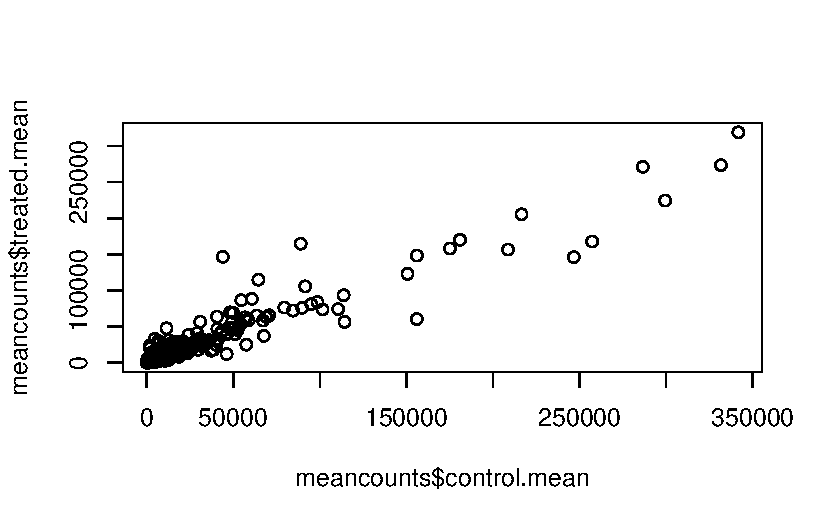
\includegraphics{class12_files/figure-pdf/unnamed-chunk-16-1.pdf}

}

\end{figure}

\begin{quote}
Q5 (b). You could also use the ggplot2 package to make this figure
producing the plot below. What geom\_?() function would you use for this
plot?
\end{quote}

The \texttt{geom\_?()} function that we can use to make this plot is
\texttt{geom\_point()}.

\begin{quote}
Q6. Try plotting both axes on a log scale. What is the argument to
plot() that allows you to do this?
\end{quote}

\begin{Shaded}
\begin{Highlighting}[]
\FunctionTok{plot}\NormalTok{(meancounts}\SpecialCharTok{$}\NormalTok{control.mean, meancounts}\SpecialCharTok{$}\NormalTok{treated.mean, }\AttributeTok{log=}\StringTok{"xy"}\NormalTok{)}
\end{Highlighting}
\end{Shaded}

\begin{verbatim}
Warning in xy.coords(x, y, xlabel, ylabel, log): 15032 x values <= 0 omitted
from logarithmic plot
\end{verbatim}

\begin{verbatim}
Warning in xy.coords(x, y, xlabel, ylabel, log): 15281 y values <= 0 omitted
from logarithmic plot
\end{verbatim}

\begin{figure}[H]

{\centering 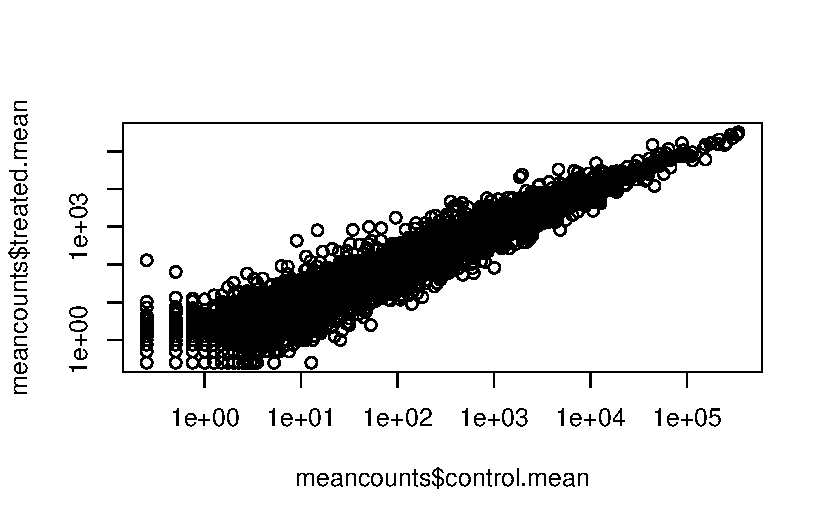
\includegraphics{class12_files/figure-pdf/unnamed-chunk-17-1.pdf}

}

\end{figure}

The argument we add to the \texttt{plot()} function that allows us to
plot both axes on a log scale is `log=``xy''.'

The most useful and most straightforward to understand is log2
transform.

\begin{Shaded}
\begin{Highlighting}[]
\FunctionTok{log2}\NormalTok{(}\DecValTok{20}\SpecialCharTok{/}\DecValTok{20}\NormalTok{)}
\end{Highlighting}
\end{Shaded}

\begin{verbatim}
[1] 0
\end{verbatim}

Doubling

\begin{Shaded}
\begin{Highlighting}[]
\FunctionTok{log2}\NormalTok{(}\DecValTok{40}\SpecialCharTok{/}\DecValTok{20}\NormalTok{)}
\end{Highlighting}
\end{Shaded}

\begin{verbatim}
[1] 1
\end{verbatim}

Half the amount

\begin{Shaded}
\begin{Highlighting}[]
\FunctionTok{log2}\NormalTok{(}\DecValTok{20}\SpecialCharTok{/}\DecValTok{40}\NormalTok{)}
\end{Highlighting}
\end{Shaded}

\begin{verbatim}
[1] -1
\end{verbatim}

\begin{Shaded}
\begin{Highlighting}[]
\FunctionTok{log2}\NormalTok{(}\DecValTok{80}\SpecialCharTok{/}\DecValTok{20}\NormalTok{)}
\end{Highlighting}
\end{Shaded}

\begin{verbatim}
[1] 2
\end{verbatim}

Add a ``log2 fold-change''.

\begin{Shaded}
\begin{Highlighting}[]
\NormalTok{meancounts}\SpecialCharTok{$}\NormalTok{log2fc }\OtherTok{\textless{}{-}} \FunctionTok{log2}\NormalTok{(meancounts}\SpecialCharTok{$}\NormalTok{treated.mean }\SpecialCharTok{/}\NormalTok{ meancounts}\SpecialCharTok{$}\NormalTok{control.mean)}
\end{Highlighting}
\end{Shaded}

\begin{Shaded}
\begin{Highlighting}[]
\FunctionTok{head}\NormalTok{(meancounts)}
\end{Highlighting}
\end{Shaded}

\begin{verbatim}
                control.mean treated.mean      log2fc
ENSG00000000003       900.75       658.00 -0.45303916
ENSG00000000005         0.00         0.00         NaN
ENSG00000000419       520.50       546.00  0.06900279
ENSG00000000457       339.75       316.50 -0.10226805
ENSG00000000460        97.25        78.75 -0.30441833
ENSG00000000938         0.75         0.00        -Inf
\end{verbatim}

Hmmm\ldots{} we need to get rid of the genes where we have no count data
as taking the log2 of these 0 counts does not tell us anything.

\begin{Shaded}
\begin{Highlighting}[]
\FunctionTok{head}\NormalTok{( meancounts }\SpecialCharTok{==} \DecValTok{0}\NormalTok{ )}
\end{Highlighting}
\end{Shaded}

\begin{verbatim}
                control.mean treated.mean log2fc
ENSG00000000003        FALSE        FALSE  FALSE
ENSG00000000005         TRUE         TRUE     NA
ENSG00000000419        FALSE        FALSE  FALSE
ENSG00000000457        FALSE        FALSE  FALSE
ENSG00000000460        FALSE        FALSE  FALSE
ENSG00000000938        FALSE         TRUE  FALSE
\end{verbatim}

\begin{Shaded}
\begin{Highlighting}[]
\NormalTok{to.keep }\OtherTok{\textless{}{-}} \FunctionTok{rowSums}\NormalTok{(meancounts[,}\DecValTok{1}\SpecialCharTok{:}\DecValTok{2}\NormalTok{] }\SpecialCharTok{==} \DecValTok{0}\NormalTok{) }\SpecialCharTok{==} \DecValTok{0}

\NormalTok{mycounts }\OtherTok{\textless{}{-}}\NormalTok{ meancounts[to.keep,]}
\FunctionTok{head}\NormalTok{(mycounts)}
\end{Highlighting}
\end{Shaded}

\begin{verbatim}
                control.mean treated.mean      log2fc
ENSG00000000003       900.75       658.00 -0.45303916
ENSG00000000419       520.50       546.00  0.06900279
ENSG00000000457       339.75       316.50 -0.10226805
ENSG00000000460        97.25        78.75 -0.30441833
ENSG00000000971      5219.00      6687.50  0.35769358
ENSG00000001036      2327.00      1785.75 -0.38194109
\end{verbatim}

\begin{Shaded}
\begin{Highlighting}[]
\CommentTok{\# nrow(mycounts)}
\end{Highlighting}
\end{Shaded}

\begin{quote}
Q7. What is the purpose of the arr.ind argument in the which() function
call above? Why would we then take the first column of the output and
need to call the unique() function?
\end{quote}

The purpose of the arr.ind argument in the \texttt{which()} function
call is to look for and return the row(s) and column(s) numbers that
contain TRUE values. In other words, it will return the row and column
numbers of where the genes (in the rows) and samples(in the columns)
have zero counts.

We need to take the first column of the output and need to call the
\texttt{unique()} function in order to make sure we are not counting any
rows that have zero counts twice in the case that there is a zero count
in both samples.

\begin{quote}
Q8. Using the up.ind vector above can you determine how many up
regulated genes we have at the greater than 2 fc level?
\end{quote}

\begin{Shaded}
\begin{Highlighting}[]
\CommentTok{\# up.ind \textless{}{-} mycounts$log2fc \textgreater{} 2}
\end{Highlighting}
\end{Shaded}

How many genes are up-regulated at the log2fc level of +2

\begin{Shaded}
\begin{Highlighting}[]
\FunctionTok{sum}\NormalTok{(mycounts}\SpecialCharTok{$}\NormalTok{log2fc }\SpecialCharTok{\textgreater{}} \SpecialCharTok{+}\DecValTok{2}\NormalTok{)}
\end{Highlighting}
\end{Shaded}

\begin{verbatim}
[1] 250
\end{verbatim}

\begin{Shaded}
\begin{Highlighting}[]
\FunctionTok{sum}\NormalTok{(mycounts}\SpecialCharTok{$}\NormalTok{log2fc }\SpecialCharTok{\textgreater{}=} \SpecialCharTok{+}\DecValTok{2}\NormalTok{)}
\end{Highlighting}
\end{Shaded}

\begin{verbatim}
[1] 314
\end{verbatim}

250 genes are up regulated at the greater than 2 fc level. 314 genes are
up regulated at the greater than or equal to 2 fc level.

\begin{quote}
Q9. Using the down.ind vector above can you determine how many down
regulated genes we have at the greater than 2 fc level?
\end{quote}

\begin{Shaded}
\begin{Highlighting}[]
\CommentTok{\# down.ind \textless{}{-} mycounts$log2fc \textless{} ({-}2)}
\end{Highlighting}
\end{Shaded}

and down-regulated\ldots{}

\begin{Shaded}
\begin{Highlighting}[]
\FunctionTok{sum}\NormalTok{(mycounts}\SpecialCharTok{$}\NormalTok{log2fc }\SpecialCharTok{\textless{}} \SpecialCharTok{{-}}\DecValTok{2}\NormalTok{)}
\end{Highlighting}
\end{Shaded}

\begin{verbatim}
[1] 367
\end{verbatim}

\begin{Shaded}
\begin{Highlighting}[]
\FunctionTok{sum}\NormalTok{(mycounts}\SpecialCharTok{$}\NormalTok{log2fc }\SpecialCharTok{\textless{}=} \SpecialCharTok{{-}}\DecValTok{2}\NormalTok{)}
\end{Highlighting}
\end{Shaded}

\begin{verbatim}
[1] 485
\end{verbatim}

367 genes are down regulated at the less than 2 fc level. 485 genes are
up regulated at the less than or equal to 2 fc level.

\begin{quote}
Q10. Do you trust these results? Why or why not?
\end{quote}

We are missing the stats. Are these big changes significant?

No, we do not trust these results. This is because we do not know if our
analysis is statistically significant (i.e.~has a p-value of less than
or equal to 0.05). When looking at fold change, change can be very large
in either direction without being statistically significant. Because we
have not done a t-test on these differences in the data, we cannot
conclude that these results are statistically significant, and
therefore, we cannot trust it.

\hypertarget{deseq2-analysis}{%
\section{DESeq2 analysis}\label{deseq2-analysis}}

\begin{Shaded}
\begin{Highlighting}[]
\FunctionTok{library}\NormalTok{(DESeq2)}
\end{Highlighting}
\end{Shaded}

Like most bioconductor packages, DESeq wants its input and output in a
very specific format.

\begin{Shaded}
\begin{Highlighting}[]
\NormalTok{dds }\OtherTok{\textless{}{-}} \FunctionTok{DESeqDataSetFromMatrix}\NormalTok{(}\AttributeTok{countData =}\NormalTok{ counts, }
                       \AttributeTok{colData =}\NormalTok{ metadata, }
                       \AttributeTok{design =} \SpecialCharTok{\textasciitilde{}}\NormalTok{dex)}
\end{Highlighting}
\end{Shaded}

\begin{verbatim}
converting counts to integer mode
\end{verbatim}

\begin{verbatim}
Warning in DESeqDataSet(se, design = design, ignoreRank): some variables in
design formula are characters, converting to factors
\end{verbatim}

The main DESeq function is called DESeq.

\begin{Shaded}
\begin{Highlighting}[]
\NormalTok{dds }\OtherTok{\textless{}{-}} \FunctionTok{DESeq}\NormalTok{(dds)}
\end{Highlighting}
\end{Shaded}

\begin{verbatim}
estimating size factors
\end{verbatim}

\begin{verbatim}
estimating dispersions
\end{verbatim}

\begin{verbatim}
gene-wise dispersion estimates
\end{verbatim}

\begin{verbatim}
mean-dispersion relationship
\end{verbatim}

\begin{verbatim}
final dispersion estimates
\end{verbatim}

\begin{verbatim}
fitting model and testing
\end{verbatim}

\begin{Shaded}
\begin{Highlighting}[]
\NormalTok{res }\OtherTok{\textless{}{-}} \FunctionTok{results}\NormalTok{(dds)}
\FunctionTok{head}\NormalTok{(res)}
\end{Highlighting}
\end{Shaded}

\begin{verbatim}
log2 fold change (MLE): dex treated vs control 
Wald test p-value: dex treated vs control 
DataFrame with 6 rows and 6 columns
                  baseMean log2FoldChange     lfcSE      stat    pvalue
                 <numeric>      <numeric> <numeric> <numeric> <numeric>
ENSG00000000003 747.194195     -0.3507030  0.168246 -2.084470 0.0371175
ENSG00000000005   0.000000             NA        NA        NA        NA
ENSG00000000419 520.134160      0.2061078  0.101059  2.039475 0.0414026
ENSG00000000457 322.664844      0.0245269  0.145145  0.168982 0.8658106
ENSG00000000460  87.682625     -0.1471420  0.257007 -0.572521 0.5669691
ENSG00000000938   0.319167     -1.7322890  3.493601 -0.495846 0.6200029
                     padj
                <numeric>
ENSG00000000003  0.163035
ENSG00000000005        NA
ENSG00000000419  0.176032
ENSG00000000457  0.961694
ENSG00000000460  0.815849
ENSG00000000938        NA
\end{verbatim}

\hypertarget{volcano-plots}{%
\section{Volcano plots}\label{volcano-plots}}

A major summary figure of this type of analysis is called a volcano plot
- the idea here is to keep out inner biologist and inner stats person
happy with one col plot!

\begin{Shaded}
\begin{Highlighting}[]
\FunctionTok{plot}\NormalTok{(res}\SpecialCharTok{$}\NormalTok{log2FoldChange, res}\SpecialCharTok{$}\NormalTok{padj)}
\end{Highlighting}
\end{Shaded}

\begin{figure}[H]

{\centering 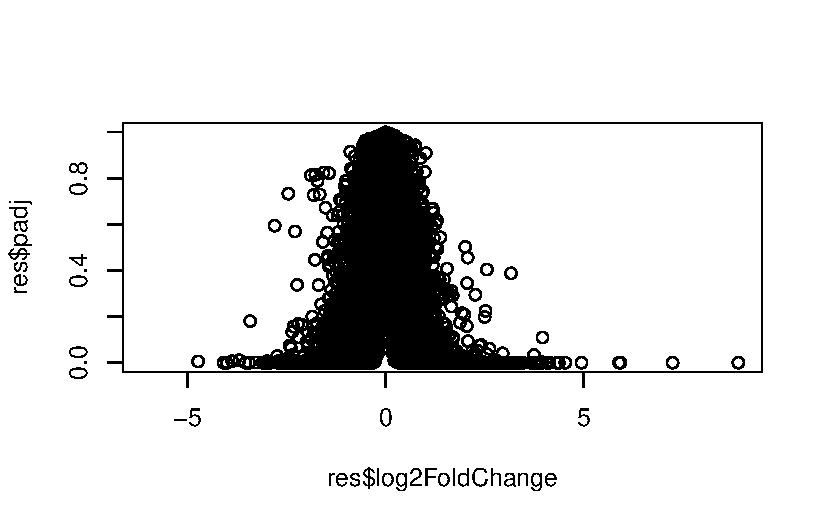
\includegraphics{class12_files/figure-pdf/unnamed-chunk-34-1.pdf}

}

\end{figure}

Improve this plot by taking the log of that p-value axis.

\begin{Shaded}
\begin{Highlighting}[]
\FunctionTok{plot}\NormalTok{(res}\SpecialCharTok{$}\NormalTok{log2FoldChange, }\FunctionTok{log}\NormalTok{(res}\SpecialCharTok{$}\NormalTok{padj))}
\end{Highlighting}
\end{Shaded}

\begin{figure}[H]

{\centering 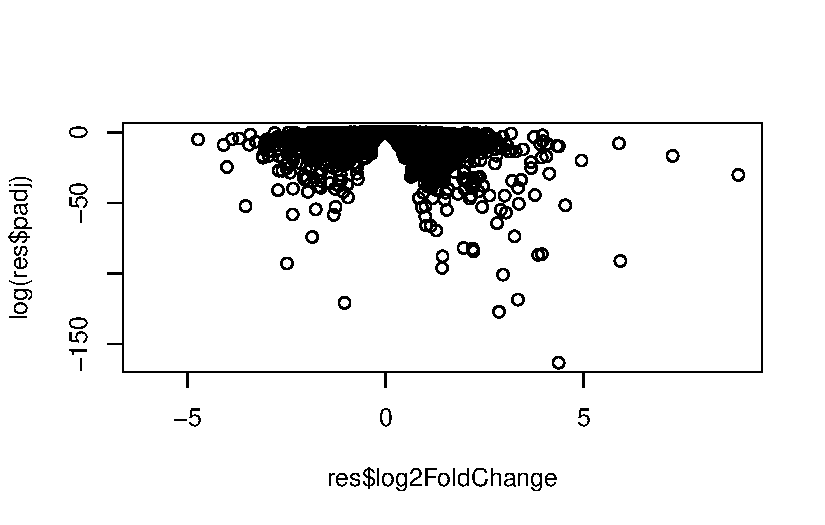
\includegraphics{class12_files/figure-pdf/unnamed-chunk-35-1.pdf}

}

\end{figure}

I want to flip this y-axis so the values I care about (i.e.~the low
p-value or high log(p-values)) are at the top of the axis.

\begin{Shaded}
\begin{Highlighting}[]
\FunctionTok{plot}\NormalTok{(res}\SpecialCharTok{$}\NormalTok{log2FoldChange, }\SpecialCharTok{{-}}\FunctionTok{log}\NormalTok{(res}\SpecialCharTok{$}\NormalTok{padj))}
\end{Highlighting}
\end{Shaded}

\begin{figure}[H]

{\centering 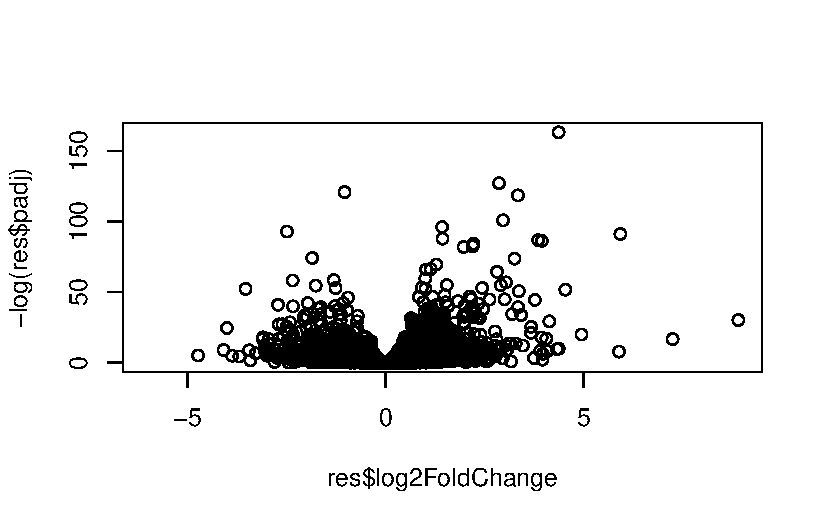
\includegraphics{class12_files/figure-pdf/unnamed-chunk-36-1.pdf}

}

\end{figure}

Let's finish up for today by adding some color to better highlight the
subset of genes that we will focus on the next day - i.e.~those with big
log2fc values (at +2/-2 threshold) and significant p-values (less than
0.05 for example).

\begin{Shaded}
\begin{Highlighting}[]
\NormalTok{mycols }\OtherTok{\textless{}{-}} \FunctionTok{rep}\NormalTok{(}\StringTok{"gray"}\NormalTok{, }\FunctionTok{nrow}\NormalTok{(res))}
\NormalTok{mycols[ }\FunctionTok{abs}\NormalTok{(res}\SpecialCharTok{$}\NormalTok{log2FoldChange) }\SpecialCharTok{\textgreater{}=} \DecValTok{2}\NormalTok{] }\OtherTok{\textless{}{-}} \StringTok{"blue"}
\NormalTok{mycols[ res}\SpecialCharTok{$}\NormalTok{padj }\SpecialCharTok{\textgreater{}} \FloatTok{0.05}\NormalTok{ ] }\OtherTok{\textless{}{-}} \StringTok{"red"}
\end{Highlighting}
\end{Shaded}

\begin{Shaded}
\begin{Highlighting}[]
\FunctionTok{plot}\NormalTok{(res}\SpecialCharTok{$}\NormalTok{log2FoldChange, }\SpecialCharTok{{-}}\FunctionTok{log}\NormalTok{(res}\SpecialCharTok{$}\NormalTok{padj), }\AttributeTok{col=}\NormalTok{mycols)}
\FunctionTok{abline}\NormalTok{(}\AttributeTok{v=}\FunctionTok{c}\NormalTok{(}\SpecialCharTok{{-}}\DecValTok{2}\NormalTok{,}\DecValTok{2}\NormalTok{), }\AttributeTok{lty=}\DecValTok{2}\NormalTok{)}
\end{Highlighting}
\end{Shaded}

\begin{figure}[H]

{\centering 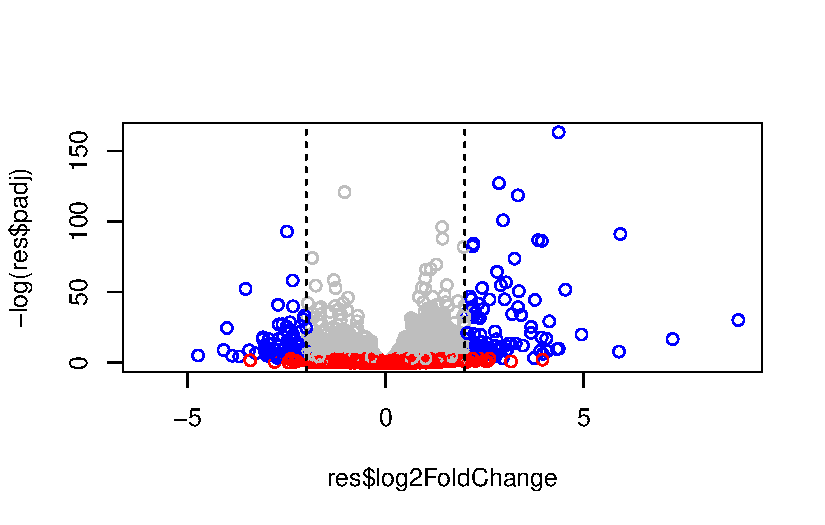
\includegraphics{class12_files/figure-pdf/unnamed-chunk-38-1.pdf}

}

\end{figure}

\begin{Shaded}
\begin{Highlighting}[]
\CommentTok{\# Setup our custom point color vector }
\NormalTok{mycols }\OtherTok{\textless{}{-}} \FunctionTok{rep}\NormalTok{(}\StringTok{"gray"}\NormalTok{, }\FunctionTok{nrow}\NormalTok{(res))}
\NormalTok{mycols[ }\FunctionTok{abs}\NormalTok{(res}\SpecialCharTok{$}\NormalTok{log2FoldChange) }\SpecialCharTok{\textgreater{}=} \DecValTok{2}\NormalTok{ ]  }\OtherTok{\textless{}{-}} \StringTok{"forestgreen"} 

\NormalTok{inds }\OtherTok{\textless{}{-}}\NormalTok{ (res}\SpecialCharTok{$}\NormalTok{padj }\SpecialCharTok{\textless{}} \FloatTok{0.01}\NormalTok{) }\SpecialCharTok{\&}\NormalTok{ (}\FunctionTok{abs}\NormalTok{(res}\SpecialCharTok{$}\NormalTok{log2FoldChange) }\SpecialCharTok{\textgreater{}} \DecValTok{2}\NormalTok{ )}
\NormalTok{mycols[ inds ] }\OtherTok{\textless{}{-}} \StringTok{"purple"}

\CommentTok{\# Volcano plot with custom colors }
\FunctionTok{plot}\NormalTok{( res}\SpecialCharTok{$}\NormalTok{log2FoldChange,  }\SpecialCharTok{{-}}\FunctionTok{log}\NormalTok{(res}\SpecialCharTok{$}\NormalTok{padj), }
 \AttributeTok{col=}\NormalTok{mycols, }\AttributeTok{ylab=}\StringTok{"{-}Log(P{-}value)"}\NormalTok{, }\AttributeTok{xlab=}\StringTok{"Log2(FoldChange)"}\NormalTok{ )}

\CommentTok{\# Cut{-}off lines}
\FunctionTok{abline}\NormalTok{(}\AttributeTok{v=}\FunctionTok{c}\NormalTok{(}\SpecialCharTok{{-}}\DecValTok{2}\NormalTok{,}\DecValTok{2}\NormalTok{), }\AttributeTok{col=}\StringTok{"gray"}\NormalTok{, }\AttributeTok{lty=}\DecValTok{2}\NormalTok{)}
\FunctionTok{abline}\NormalTok{(}\AttributeTok{h=}\SpecialCharTok{{-}}\FunctionTok{log}\NormalTok{(}\FloatTok{0.1}\NormalTok{), }\AttributeTok{col=}\StringTok{"gray"}\NormalTok{, }\AttributeTok{lty=}\DecValTok{2}\NormalTok{)}
\end{Highlighting}
\end{Shaded}

\begin{figure}[H]

{\centering 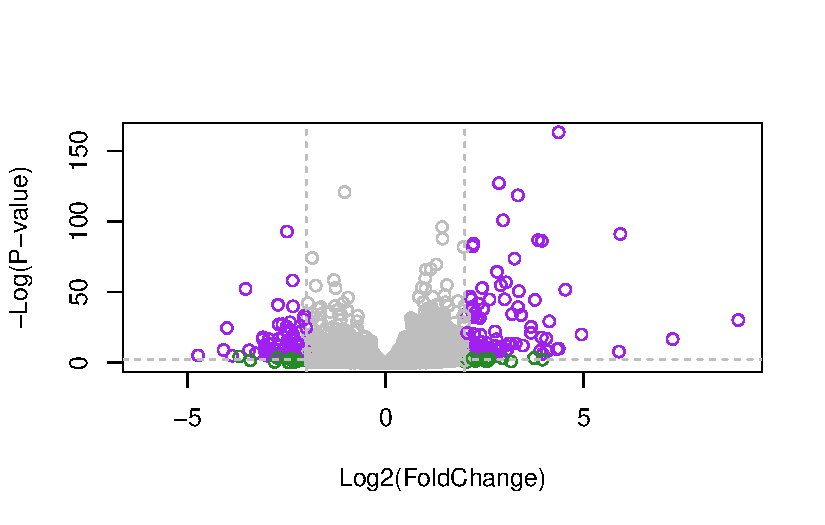
\includegraphics{class12_files/figure-pdf/unnamed-chunk-39-1.pdf}

}

\end{figure}

\hypertarget{gene-annotation}{%
\subsection{Gene annotation}\label{gene-annotation}}

We will use one of Bioconductor's main annotation packages to help with
mapping between various ID schemes. Here, we load the
\texttt{AnnotationDbi} package and the annotation package for humans
\texttt{org.Hs.eg.db}.

\begin{Shaded}
\begin{Highlighting}[]
\FunctionTok{head}\NormalTok{(res)}
\end{Highlighting}
\end{Shaded}

\begin{verbatim}
log2 fold change (MLE): dex treated vs control 
Wald test p-value: dex treated vs control 
DataFrame with 6 rows and 6 columns
                  baseMean log2FoldChange     lfcSE      stat    pvalue
                 <numeric>      <numeric> <numeric> <numeric> <numeric>
ENSG00000000003 747.194195     -0.3507030  0.168246 -2.084470 0.0371175
ENSG00000000005   0.000000             NA        NA        NA        NA
ENSG00000000419 520.134160      0.2061078  0.101059  2.039475 0.0414026
ENSG00000000457 322.664844      0.0245269  0.145145  0.168982 0.8658106
ENSG00000000460  87.682625     -0.1471420  0.257007 -0.572521 0.5669691
ENSG00000000938   0.319167     -1.7322890  3.493601 -0.495846 0.6200029
                     padj
                <numeric>
ENSG00000000003  0.163035
ENSG00000000005        NA
ENSG00000000419  0.176032
ENSG00000000457  0.961694
ENSG00000000460  0.815849
ENSG00000000938        NA
\end{verbatim}

\begin{Shaded}
\begin{Highlighting}[]
\CommentTok{\# rownames(res)}
\end{Highlighting}
\end{Shaded}

\begin{Shaded}
\begin{Highlighting}[]
\CommentTok{\# BiocManager::install("AnnotationDbi")}
\CommentTok{\# BiocManager::install("org.Hs.eg.db")}

\FunctionTok{library}\NormalTok{(}\StringTok{"AnnotationDbi"}\NormalTok{)}
\FunctionTok{library}\NormalTok{(}\StringTok{"org.Hs.eg.db"}\NormalTok{)}
\end{Highlighting}
\end{Shaded}

\begin{verbatim}
\end{verbatim}

Look at what types of IDs I can translate between from the the
\texttt{org.Hs.eg.db} package with the \texttt{columns()} function.

\begin{Shaded}
\begin{Highlighting}[]
\FunctionTok{columns}\NormalTok{(org.Hs.eg.db)}
\end{Highlighting}
\end{Shaded}

\begin{verbatim}
 [1] "ACCNUM"       "ALIAS"        "ENSEMBL"      "ENSEMBLPROT"  "ENSEMBLTRANS"
 [6] "ENTREZID"     "ENZYME"       "EVIDENCE"     "EVIDENCEALL"  "GENENAME"    
[11] "GENETYPE"     "GO"           "GOALL"        "IPI"          "MAP"         
[16] "OMIM"         "ONTOLOGY"     "ONTOLOGYALL"  "PATH"         "PFAM"        
[21] "PMID"         "PROSITE"      "REFSEQ"       "SYMBOL"       "UCSCKG"      
[26] "UNIPROT"     
\end{verbatim}

\begin{Shaded}
\begin{Highlighting}[]
\NormalTok{res}\SpecialCharTok{$}\NormalTok{symbol }\OtherTok{\textless{}{-}} \FunctionTok{mapIds}\NormalTok{(}\AttributeTok{x=}\NormalTok{org.Hs.eg.db,}
                    \AttributeTok{column =} \StringTok{"SYMBOL"}\NormalTok{,}
                    \AttributeTok{keys =} \FunctionTok{rownames}\NormalTok{(res),}
                    \AttributeTok{keytype =} \StringTok{"ENSEMBL"}\NormalTok{)}
\end{Highlighting}
\end{Shaded}

\begin{verbatim}
'select()' returned 1:many mapping between keys and columns
\end{verbatim}

\begin{quote}
Q11. Run the mapIds() function two more times to add the Entrez ID and
UniProt accession and GENENAME as new columns called
res\(entrez, res\)uniprot and res\$genename.
\end{quote}

\begin{Shaded}
\begin{Highlighting}[]
\NormalTok{res}\SpecialCharTok{$}\NormalTok{entrez }\OtherTok{\textless{}{-}} \FunctionTok{mapIds}\NormalTok{(}\AttributeTok{x=}\NormalTok{org.Hs.eg.db,}
                     \AttributeTok{column =} \StringTok{"ENTREZID"}\NormalTok{,}
                     \AttributeTok{keys =} \FunctionTok{rownames}\NormalTok{(res),}
                     \AttributeTok{keytype =} \StringTok{"ENSEMBL"}\NormalTok{)}
\end{Highlighting}
\end{Shaded}

\begin{verbatim}
'select()' returned 1:many mapping between keys and columns
\end{verbatim}

\begin{Shaded}
\begin{Highlighting}[]
\NormalTok{res}\SpecialCharTok{$}\NormalTok{uniprot }\OtherTok{\textless{}{-}} \FunctionTok{mapIds}\NormalTok{(}\AttributeTok{x=}\NormalTok{org.Hs.eg.db,}
                    \AttributeTok{column =} \StringTok{"UNIPROT"}\NormalTok{,}
                    \AttributeTok{keys =} \FunctionTok{rownames}\NormalTok{(res),}
                    \AttributeTok{keytype =} \StringTok{"ENSEMBL"}\NormalTok{)}
\end{Highlighting}
\end{Shaded}

\begin{verbatim}
'select()' returned 1:many mapping between keys and columns
\end{verbatim}

\begin{Shaded}
\begin{Highlighting}[]
\NormalTok{res}\SpecialCharTok{$}\NormalTok{genename }\OtherTok{\textless{}{-}} \FunctionTok{mapIds}\NormalTok{(}\AttributeTok{x=}\NormalTok{org.Hs.eg.db,}
                       \AttributeTok{column =} \StringTok{"GENENAME"}\NormalTok{,}
                       \AttributeTok{keys =} \FunctionTok{rownames}\NormalTok{(res),}
                       \AttributeTok{keytype =} \StringTok{"ENSEMBL"}\NormalTok{)}
\end{Highlighting}
\end{Shaded}

\begin{verbatim}
'select()' returned 1:many mapping between keys and columns
\end{verbatim}

\hypertarget{pathway-analysis}{%
\section{Pathway Analysis}\label{pathway-analysis}}

We will finish this lab witha quick pathway analysis. Here, we play iwth
just the \textbf{GAGE package} (Which stands for Generally Applicable
Gene set Enrichment), to do \textbf{KEGG pathway Enrichment analysis} on
our RNA-seq based differential expression results.

\begin{Shaded}
\begin{Highlighting}[]
\CommentTok{\# BiocManager::install( c("pathview", "gage", "gageData") )}
\end{Highlighting}
\end{Shaded}

\begin{Shaded}
\begin{Highlighting}[]
\FunctionTok{library}\NormalTok{(pathview)}
\end{Highlighting}
\end{Shaded}

\begin{verbatim}
##############################################################################
Pathview is an open source software package distributed under GNU General
Public License version 3 (GPLv3). Details of GPLv3 is available at
http://www.gnu.org/licenses/gpl-3.0.html. Particullary, users are required to
formally cite the original Pathview paper (not just mention it) in publications
or products. For details, do citation("pathview") within R.

The pathview downloads and uses KEGG data. Non-academic uses may require a KEGG
license agreement (details at http://www.kegg.jp/kegg/legal.html).
##############################################################################
\end{verbatim}

\begin{Shaded}
\begin{Highlighting}[]
\FunctionTok{library}\NormalTok{(gage)}
\end{Highlighting}
\end{Shaded}

\begin{verbatim}
\end{verbatim}

\begin{Shaded}
\begin{Highlighting}[]
\FunctionTok{library}\NormalTok{(gageData)}

\FunctionTok{data}\NormalTok{(kegg.sets.hs)}

\CommentTok{\# Examine the first 2 pathways in this kegg set for humans}
\FunctionTok{head}\NormalTok{(kegg.sets.hs, }\DecValTok{2}\NormalTok{)}
\end{Highlighting}
\end{Shaded}

\begin{verbatim}
$`hsa00232 Caffeine metabolism`
[1] "10"   "1544" "1548" "1549" "1553" "7498" "9"   

$`hsa00983 Drug metabolism - other enzymes`
 [1] "10"     "1066"   "10720"  "10941"  "151531" "1548"   "1549"   "1551"  
 [9] "1553"   "1576"   "1577"   "1806"   "1807"   "1890"   "221223" "2990"  
[17] "3251"   "3614"   "3615"   "3704"   "51733"  "54490"  "54575"  "54576" 
[25] "54577"  "54578"  "54579"  "54600"  "54657"  "54658"  "54659"  "54963" 
[33] "574537" "64816"  "7083"   "7084"   "7172"   "7363"   "7364"   "7365"  
[41] "7366"   "7367"   "7371"   "7372"   "7378"   "7498"   "79799"  "83549" 
[49] "8824"   "8833"   "9"      "978"   
\end{verbatim}

The main \texttt{gage()} function requires a named vector of fold
changes, where the names of the values are the Entrez gene IDs.

\begin{Shaded}
\begin{Highlighting}[]
\FunctionTok{c}\NormalTok{(}\AttributeTok{barry=}\DecValTok{4}\NormalTok{, }\AttributeTok{clair=}\DecValTok{3}\NormalTok{, }\AttributeTok{chandra=}\DecValTok{2}\NormalTok{)}
\end{Highlighting}
\end{Shaded}

\begin{verbatim}
  barry   clair chandra 
      4       3       2 
\end{verbatim}

\begin{Shaded}
\begin{Highlighting}[]
\NormalTok{foldchanges }\OtherTok{\textless{}{-}}\NormalTok{ res}\SpecialCharTok{$}\NormalTok{log2FoldChange}
\FunctionTok{names}\NormalTok{(foldchanges) }\OtherTok{\textless{}{-}}\NormalTok{ res}\SpecialCharTok{$}\NormalTok{entrez}

\FunctionTok{head}\NormalTok{(foldchanges)}
\end{Highlighting}
\end{Shaded}

\begin{verbatim}
       7105       64102        8813       57147       55732        2268 
-0.35070302          NA  0.20610777  0.02452695 -0.14714205 -1.73228897 
\end{verbatim}

Now, let's run the gage pathway analysis.

\begin{Shaded}
\begin{Highlighting}[]
\CommentTok{\# Get the results}
\NormalTok{keggres }\OtherTok{=} \FunctionTok{gage}\NormalTok{(foldchanges, }\AttributeTok{gsets=}\NormalTok{kegg.sets.hs)}
\end{Highlighting}
\end{Shaded}

Now lets look at the object returned from \texttt{gage()}, i.e.~our
results here:

\begin{Shaded}
\begin{Highlighting}[]
\FunctionTok{attributes}\NormalTok{(keggres)}
\end{Highlighting}
\end{Shaded}

\begin{verbatim}
$names
[1] "greater" "less"    "stats"  
\end{verbatim}

\begin{Shaded}
\begin{Highlighting}[]
\CommentTok{\# Look at the first three down (less) pathways}
\FunctionTok{head}\NormalTok{(keggres}\SpecialCharTok{$}\NormalTok{less, }\DecValTok{3}\NormalTok{)}
\end{Highlighting}
\end{Shaded}

\begin{verbatim}
                                      p.geomean stat.mean        p.val
hsa05332 Graft-versus-host disease 0.0004250461 -3.473346 0.0004250461
hsa04940 Type I diabetes mellitus  0.0017820293 -3.002352 0.0017820293
hsa05310 Asthma                    0.0020045888 -3.009050 0.0020045888
                                        q.val set.size         exp1
hsa05332 Graft-versus-host disease 0.09053483       40 0.0004250461
hsa04940 Type I diabetes mellitus  0.14232581       42 0.0017820293
hsa05310 Asthma                    0.14232581       29 0.0020045888
\end{verbatim}

Let's pull up the highlighted pathway and show our differentially
expressed genes on the pathway. I will use the ``hsa'' KEGG id to get
the pathway from KEGG and my \texttt{foldchange} vector to show my
genes.

\begin{Shaded}
\begin{Highlighting}[]
\FunctionTok{pathview}\NormalTok{(}\AttributeTok{gene.data=}\NormalTok{foldchanges, }\AttributeTok{pathway.id=}\StringTok{"hsa05310"}\NormalTok{, }\AttributeTok{kegg.native=}\ConstantTok{FALSE}\NormalTok{)}
\end{Highlighting}
\end{Shaded}

\begin{verbatim}
'select()' returned 1:1 mapping between keys and columns
\end{verbatim}

\begin{verbatim}
Info: Working in directory C:/Users/Olivia Chu/Documents/UCSD/Senior (2022-23)/Winter 2023/BIMM 143 (Grant)/class12
\end{verbatim}

\begin{verbatim}
Info: Writing image file hsa05310.pathview.pdf
\end{verbatim}

Put this into my document.

\begin{figure}

{\centering 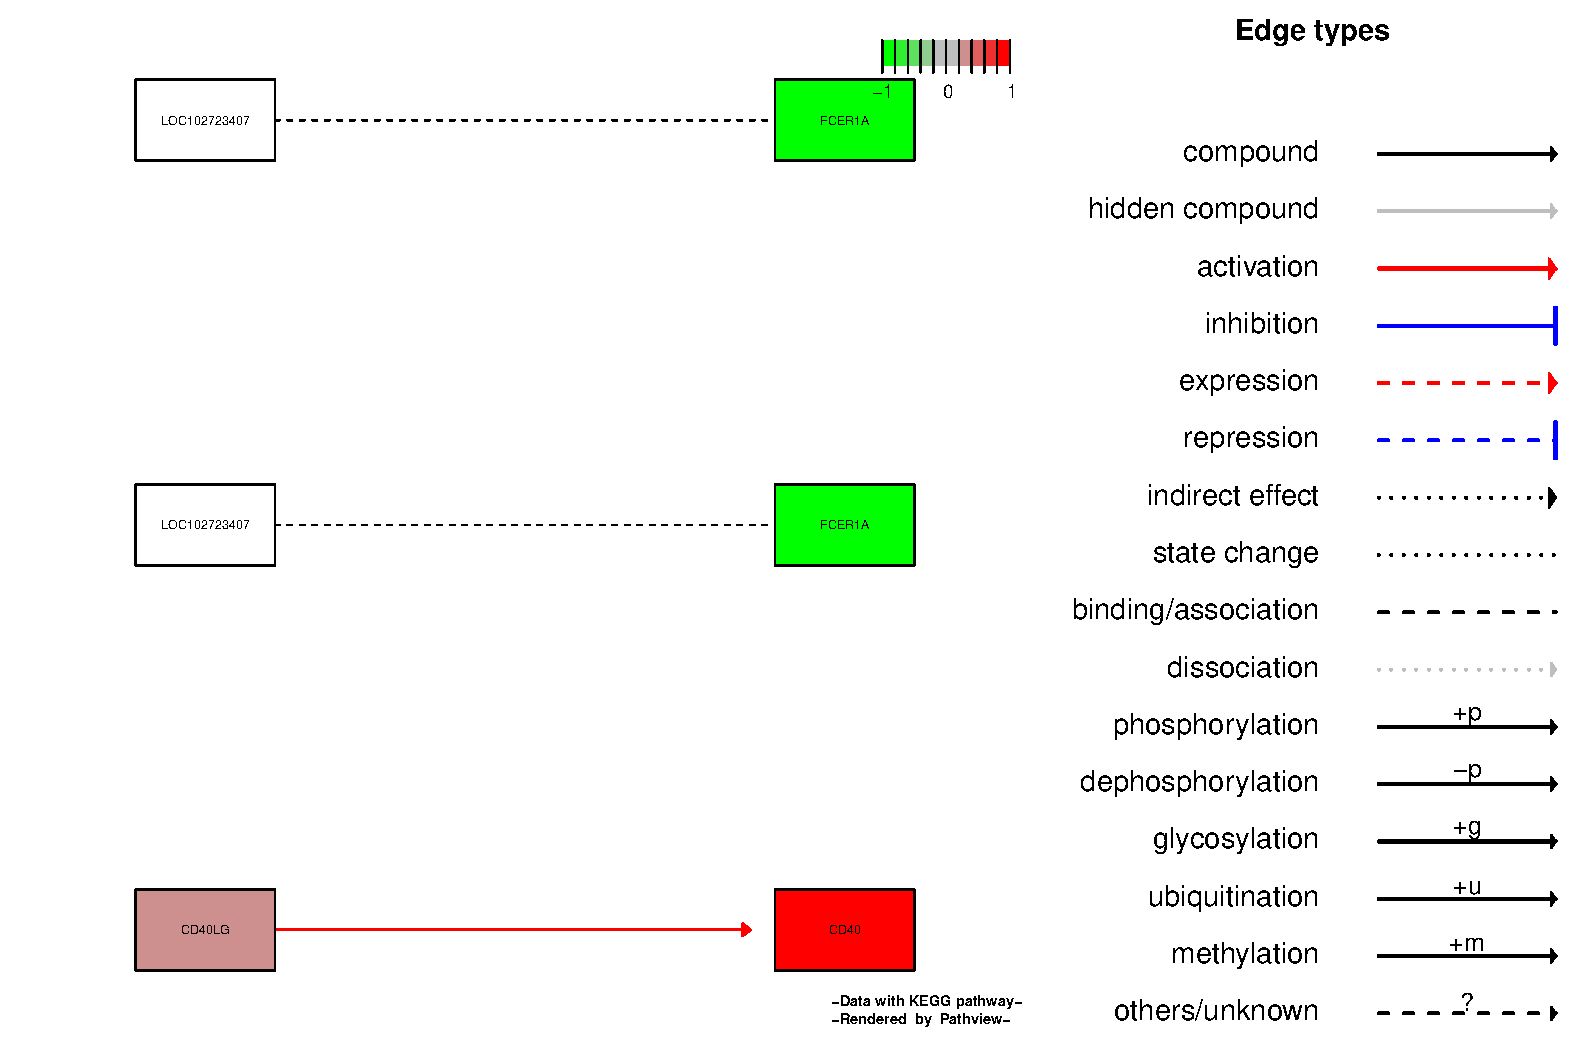
\includegraphics{hsa05310.pathview.png}

}

\caption{The Asthma pathway with my highlighted differentially expressed
genes in color}

\end{figure}



\end{document}
